\documentclass{article}
\usepackage{multicol}
\usepackage{graphicx}% Include figure files
\usepackage{dcolumn}% Align table columns on decimal point
\usepackage{bm}% bold math
\usepackage{hyperref}% add hypertext capabilities
\usepackage{booktabs}
\usepackage{listings}
\usepackage{mathtools}
\usepackage{amsmath}
\renewcommand{\abstractname}{\vspace{-\baselineskip}}
\bibliographystyle{plain}
\usepackage[utf8]{inputenc}
\usepackage{verbatim} %for å inkludere filer med tegn LaTeX ikke liker
\usepackage{mathpazo}
\usepackage{float}
\usepackage{algpseudocode}
\newcommand\numberthis{\addtocounter{equation}{1}\tag{\theequation}}
\usepackage[left=20mm,right=20mm,top=33.95mm,bottom=33.95mm]{geometry} 
% Justerer bredden på columns.
\setlength{\columnsep}{1cm}

\begin{document}

\title{The ising model}
\author{Sebastian Amundsen, Marcus Berget and Andreas Wetzel}

\maketitle

\begin{abstract}

\end{abstract}

\begin{multicols}{2}

\section{Introduction}

There are many different models for simulating the world of statistical mechanics, each with their respective pros and cons. However, there are few, if any, that can match the simplicity of the Ising model while at the same time showing phase transitions. In this project we will explore the Ising model, with the final aim of reproducing its critical temperature of the the phase transition. We will first start by simulating the Ising model, assuming a square 2 x 2 lattice. The analytical expressions for the expectation values of the energy and mean absolute magnetization for this specific system are known, and will serve as a great benchmark for testing whether we have implemented the model correctly. Once the simulated results reaches a good agreement with the analytical ones, we will extend the model to a 20 x 20 system. Here we will find the so-called burn-in time for the system, i.e., how many Monte Carlo cycles are needed before the system reaches equilibrium and we can 'safely' start computing the expectation values. We will then analyze the probability distribution for the energy of the system at $T=1.0$ and $T=2.4$, disregarding the values from the burn-in time. Finally, we will study the phase transition of the Ising model in the temperature interval between $T\in[2.0, 2.3]$. In order to estimate the critical temperature $T_C$ of the phase transition we will vary the lattice size and use small temperature steps in our simulation, causing relatively long simulation times.


\section{Theory}

\subsection*{Canonical Ensemble}
In statistical physics you represent the possible states of systems by ensembles, which are collections of microscopic systems from which we can derive expectation values and thermodynamic properties related to an experiment \cite{95}. For the Ising model we will use a canonical ensemble in order to calculate various expectation values such as the mean energy. 

The partition function for the canonical ensemble is given by:

\begin{equation}
Z(\beta) = \sum_{s} e^{(-\beta E_s)}
\label{eq:Z}
\end{equation}

With $\beta=1/k_BT$, where T is temperature, $k_B$ is Boltzmann's constant and $E_s$ is the energy in a given state. We can use this partition function to find the probability $P_s$ of finding a system in a state s:

\begin{equation}
P_s=\frac{e^{-(\beta E_s)}}{Z}
\label{eq:P_s}
\end{equation}

Furthermore, the mean energy $\langle E \rangle$ can be calculated using the probability distribution $P_s$, We then have that the mean energy  is given by:

\begin{equation}
\langle E \rangle = \sum_s E_s P_s(\beta)  = \sum_s \frac{E_s e^{-(\beta*E_s)}}{Z}
\label{eq:E_m}
\end{equation}

The variance $\sigma_E^2$ corresponding to the mean energy is defined as:

\begin{equation}
\begin{split}
\sigma_E^2 &= \langle E^2 \rangle - \langle E \rangle^2 \\
&= \sum_s \frac{E_s^2 e^{-(\beta*E_s)}}{Z} - \bigg(\sum_s \frac{E_s e^{-(\beta*E_s)}}{Z}\bigg)^2
\end{split}
\label{eq:E_v}
\end{equation}

Dividing the variance by $k_bT^2$ gives rise to the heat capacity at constant volume $C_v$.

\begin{equation}
C_v = \frac{1}{kT} \sigma_E^2 
\label{eq:C_v}
\end{equation}

Just as for the mean energy, the mean magnetization $\langle M \rangle$ can be found using the probability distribution $P_s(\beta)$.

\begin{equation}
\langle M \rangle=\sum_s^M M_s P_s(\beta)=\frac{1}{Z}\sum_s^M M_s e^{-(\beta E_s)}
\label{eq:mM}
\end{equation}

Where $M_s$ are the different magnetizations. The corresponding magnetic variance is defined as

\begin{equation}
\begin{split}
\sigma_M^2&=\langle M^2 \rangle-\langle M \rangle^2 \\
& = \frac{1}{Z}\sum_s^M M_s^2 e^{-(\beta E_s)}
\end{split}
\label{eq:M_v}
\end{equation}

Finally, dividing the magnetic variance with $k_B T$ gives rise to the susceptibility $\chi$.

\begin{equation}
\chi = \frac{1}{k_BT}\sigma_M^2
\label{eq:chi}
\end{equation}


\section{Method}

\subsection*{Specific case for a 2 X 2 lattice}

We can use our analytical expressions in conjunction with some periodic boundary conditions. We assume two spins in each dimension L=2. If we draw up each lattice with the different spin orientations we can find the degeneracy, energy and magnetization for each state. These values can be used to find the analytical expressions with periodic boundary conditions. We have five different spin orientations if we are studying the spin structures in Figure \ref{fig:spinn}. The energy differences $\Delta E$ in such a structure is given by:

\begin{equation}
\Delta E = E_2 - E_1 =  2J s_l^1\sum_{<k>}^N s_k
\label{eq:dE}
\end{equation}

where $E_2$ is the energy after, $E_1$ the energy before and the sum runs  over the nearest neighbors k of spin l. We can also find the difference in magnetization $\Delta M$ by only flipping the spin in the middle (dot in Figure \ref{fig:spinn}):

\begin{equation}
\Delta M = M_2-M_1=\pm2
\label{eq:dM}
\end{equation}

Where $M_2$ is the magnetization after and $M_1$ is the magnetization before we flip the spin. We can see that the change in magnetization is always $\Delta M=\pm2$, given that we only have spin configurations L=$\pm1$. These expressions are only valid as long as we have zero magnetic field. 

\subsection*{The ising model}

The square lattice Ising model is a simple statistical model, which can be used to show phase transitions. We run through the lattice using the Monte Carlo algorithm.

For every Monte Carlo cycle 


\subsection*{Metropolis algorithm}

We wish to find the energy differences and the change in magnetization as we run through our simulation. It is beneficial to find the energy differences before we do the metropolis sampling. Since we are only flipping one spin at a time, it is possible to find and store all the energy differences in an array as $e^{\beta\Delta E}$. This saves a lot of time, as we don't have to evaluate the exponentials in the Monte Carlo sampling. 

The metropolis algorithm only considers ratios between probabilities, which means that we do not need to calculate the partition function at all when we are using the algorithm \cite{94}. 

\subsection*{Expectation values given the number of Monte Carlo cycles}

We want to study how many Monte Carlo cycles we need before we reach a equilibrium state. This is given when the expectation values start to stabilize at a set number of Monte Carlo cycles. When we have reached this equilibrium situation we can start to extract more realistic expectation values. We find the equilibrium point by plotting the expectation values as a function of the number of Monte Carlo cycles and study where the values begin to stabilize. The number of Monte Carlo cycles before we reach the equilibrium is called the burn-in time for the system. We can now find a probability distribution for the energy of the system at a set temperature. We study a $20\times20$ lattice with the temperatures T=1 and T=2.4, where the expectation values at the burnout time are disregarded. 


\section{Results}

\subsection*{Specific case for a 2 X 2 lattice}

\begin{table}[H]
\begin{center}
\caption{Energy and magnetization given number of up spins.}
\begin{tabular}{  |c|c|c|c|c|c| } \hline
$N_{\text{spins up}}$&Degeneracy&E&M \\ \hline
4&1&-8 J&4\\ \hline
3&4&0 &2 \\ \hline
2&4&0&0\\ \hline
2&2&8 J&0\\ \hline
1&4&0&-2\\ \hline
0&1&-8 J&-4\\ \hline
\end{tabular}
\label{tab:up_spins}
\end{center}
\end{table}

In Table \ref{tab:up_spins} we have the energy and magnetization given the number of up spins. 

\begin{equation}
Z=4\cosh{(8J\beta)}+12
\label{eq:Z_22}
\end{equation}

We have that the partition function for our specific $2\times2$ lattice case is given by equation \ref{eq:Z_22}.

\begin{equation}
E_m=\frac{-32J\sinh{(8J\beta)}}{Z}
\label{eq:E_22}
\end{equation}

The mean energy is given by equation \ref{eq:E_22}.

\begin{equation}
\begin{split}
C_v = \frac{1}{kTZ^2} \bigg(1024\beta J^2(3\cosh(8J\beta) + 1\bigg)
\end{split}
\label{eq:Cv_22}
\end{equation}

The heat capacity is given by equation \ref{eq:Cv_22}.

\begin{equation}
\langle M \rangle=0
\label{eq:M_22}
\end{equation}

The mean magnetization is given by equation \ref{eq:M_22}.

\begin{equation}
\chi = \frac{1}{kT} \bigg(\frac{32}{Z}(1+e^{8J\beta})-\frac{64}{Z^2}(e^{8J\beta}+2)^2\bigg)
\label{eq:chi_22}
\end{equation}

The susceptibility is given by equation \ref{eq:chi_22}. All the calculations are given in appendix B.

In the $2\times2$ lattice case there are only five possible values for the energy difference. These are given in section \ref{eq:calc_dE} in appendix B. 

\begin{figure}[H]
	\centering
	\includegraphics[width=\linewidth]{Exp_values_2x2_5e5.png}
	\caption{Analytical vs numerical for 2x2 lattice. }
	\label{fig:exp_val}
\end{figure}

In Figure \ref{fig:exp_val} we have the numerical values for energy, magnetization, heat capacity and susceptibility compared with the analytical expressions for a $2\times2$ lattice. 

\subsection*{Equilibration time and probability distribution}

\begin{figure}[H]
	\centering
	\includegraphics[width=\linewidth]{Uni_vs_rand.png}
	\caption{The mean energy and mean absolute magnetization.}
	\label{fig:mean_em}
\end{figure}

The mean energy and mean absolute magnetization as a function of the temperature T=1 and T=2.4, with uniform and random initial spin conditions is given in Figure \ref{fig:mean_em}. 

\begin{figure}[H]
	\centering
	\includegraphics[width=\linewidth]{Diff_vs_mcs.png}
	\caption{Difference as a function of Monte Carlo cycles for $2\times2$ lattice.}
	\label{fig:diff_mc}
\end{figure}

For the $2\times2$ lattice we have plotted the difference between numerical and analytical values as a function of Monte Carlo cycles in Figure \ref{fig:diff_mc}. 

\begin{figure}[H]
	\centering
	\includegraphics[width=\linewidth]{n_flips_1.png}
	\caption{Number of total accepted flips as a function of MCS for the temperature T=1.0.}
	\label{fig:n1}
\end{figure}

\begin{figure}[H]
	\centering
	\includegraphics[width=\linewidth]{n_flips_24.png}
	\caption{Number of total accepted flips as a function of MCS for the temperature T=2.4.}
	\label{fig:n24}
\end{figure}

The number of total accepted flips for the temperatures T=1.0 and T=2.4 are given in Figure \ref{fig:n1} and Figure \ref{fig:n24} respectively. 

\begin{figure}[H]
	\centering
	\includegraphics[width=\linewidth]{Hist_1.png}
	\caption{The probability distribution for the temperature T=1.0.}
	\label{fig:pd1}
\end{figure}

\begin{figure}[H]
	\centering
	\includegraphics[width=\linewidth]{Hist_24.png}
	\caption{The probability distribution for the temperature T=2.4.}
	\label{fig:pd24}
\end{figure}

We have the probability distributions for the temperatures T=1.0 and T=2.4 in Figure \ref{fig:pd1} and Figure \ref{fig:pd24} respectively. 

\subsection*{Phase transition and critical temperature}

\begin{figure}[H]
	\centering
	\includegraphics[width=\linewidth]{Exp_values.png}
	\caption{Expectation values for E, $|M|$, $C_V$ and $\chi$ as functions of T for L=40, L=60, L=80 and L=10.}
	\label{fig:exp}
\end{figure}

We have the expectation values at different lattice size in Figure \ref{fig:exp}.

\begin{figure}[H]
	\centering
	\includegraphics[width=\linewidth]{Exp_values_zoom.png}
	\caption{Heat capacity as a function of temperature over the critical temperature interval.}
	\label{fig:C_T}
\end{figure}

We have plotted the heat capacity as a function of a small temperature interval for different lattice sizes (L=40,60,80,100) in Figure \ref{fig:C_T}. 

\section{Discussion}

\subsection{$2\times 2$ lattice}

Looking at the behavior of the energy and mean absolute magnetization in Figure \ref{fig:exp_val}, there are no big surprises. We expect the total energy of the system to increase as we increase the temperature, and the mean absolute magnetization to decrease as the temperature increases. As for the behavior of the heat capacity and susceptibility, our intuition isn't as solid as to what should happen. However, it is reassuring that the data follows all the analytical expressions, indicating that our code works correctly. In addition, it is interesting to note that both the heat capacity and the susceptibility has their maximum values around $T\in[2.5, 3.0]$, which may hint to something special happening around that temperature interval (we'll come back to this). There is also a point to make around how we evaluate the burn-in time for this system. 

\subsection{$20\times 20$ lattice}

As far as our understanding goes it isn't obvious that the burn-in time for the $20 \times 20$ lattice should be the same as for the $2 \times 2$ lattice. However, we found that the burn-in times for the two systems are quite equal. This is something that we perhaps should've looked into further, testing what the burn-in time for several more lattice sizes.  Additionally, we can see that just like for the $2 \times 2$ lattice, the energy and mean absolute magnetization has more or less equal burn-in times. This makes sense, given the fact that the magnetization is a function of the energy, so when the energy stabilizes the magnetization has to as well. 

It is also interesting to see the difference between the ordered and randomized initial states at $T=1.0$ in Figure \ref{fig:mean_em}. For the ordered states, the mean energy and absolute magnetization stays constant, which makes sense given that the system is already then in its lowest possible energy state. In contrast, the mean absolute magnetization for the random state starts out at almost zero, before it quickly rises and starts converging towards 1. This isn't surprising at all, given the fact that when the initial state is fully random, there is an equal chance for the states being spin up as for it to be spin down, equalizing the total magnetization. Then, since the metropolis algorithm seeks to lower the energy of the system to the lowest possible state, the energy naturally goes down until it reaches the lowest state. For $T=2.4$ we can see that for both the ordered states and the random states, the mean energy and the mean absolute magnetization starts out at different starting points, but quickly start following the same path. We find it a little surprising that they start following the same path as much as they do, given the completely different initial states. It is true that the higher temperature will make the spins flip more often, but we can't see why this would make the states follow the seemingly exact same path. 

The difference in the probability distributions for the two different temperatures is quite noteworthy. Firstly, we note that the mean energy variance is more than 3000 times larger for the system at $T=2.4$ than for the system at $T=1$. Obviously, this means that the energy at $T=1.0$ varies much less than the energy at $T=2.4$. We can in other words pinpoint the energy of the system at $T=1.0$, with much greater confidence than for the system at $T=2.4$. Another interesting observation is that for the $T=1.0$ system, there is no weight at the energy of $-1.99$ J. This makes sense. As shown in Appendix B, the lowest possible change in energy from flipping on single spin is -4 J. 

As we have mentioned above, we estimated the burn-in time graphically. We did try to think of ways to do this more precisely by some sort of numerical estimation, but we couldn't come up with a condition that rigorously defined when the system had reached equilibrium. This could probably be done by saying that the system reaches equilibrium when the variance in expectation values goes under a given tolerance. However, we were unsure what this tolerance should have been and decided that estimating the burn-in time graphically was precise enough. After all, evaluating say 1e5 data points from the burn-in time with a total MCC of 1e6 should have very little effect on the expectation values anyway.

\section{Concluding remarks}

\end{multicols}

\clearpage

\appendix % Her kommer appendix.

\section{Appendix}

\begin{figure}[H]
	\centering
	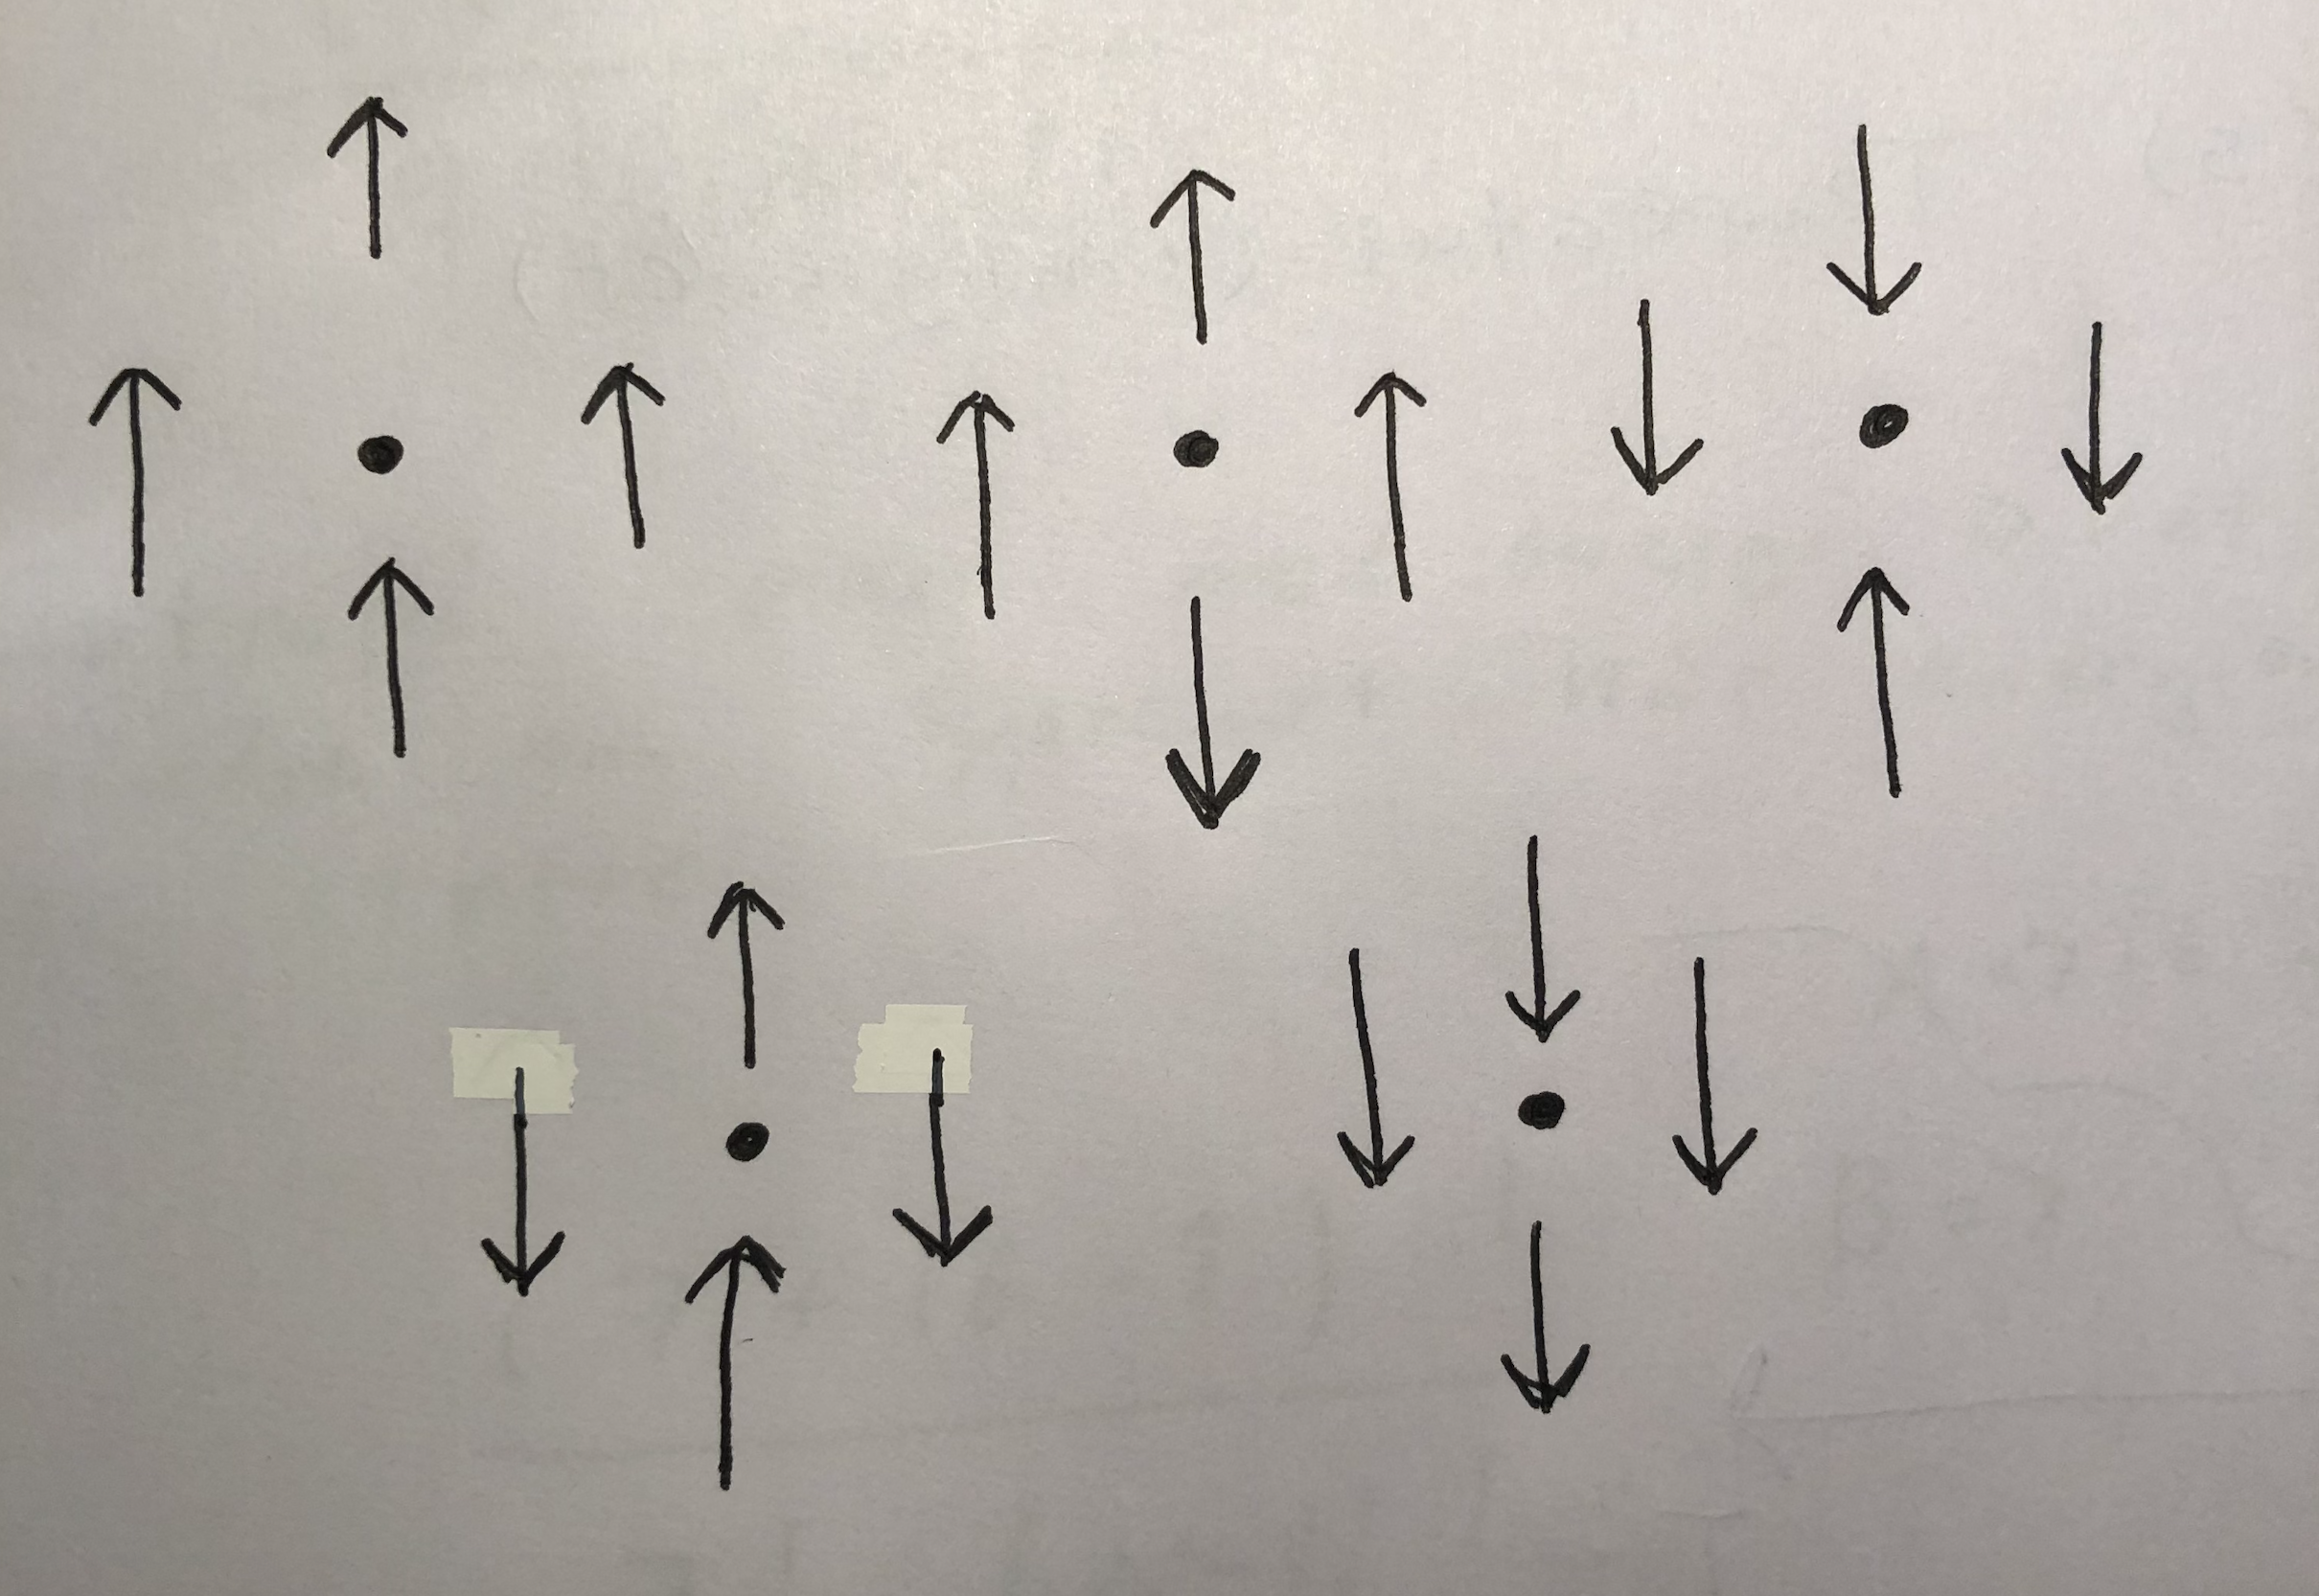
\includegraphics[width=100mm]{Spin}
	\caption{The different spin orientations.}
	\label{fig:spinn}
\end{figure}

\section{Appendix}
\subsection*{Analytical expression}

The partition function for the $2\times2$ lattice is given by equation \ref{eq:Z}:

\begin{equation}
\begin{split}
Z&=2e^{8J\beta}+2e^{-8J\beta}+12e^0\\
&=4\cosh{(8J\beta)}+12
\end{split}
\label{eq:calc_Z}
\end{equation}

This expression combined with equation \ref{eq:E_m} gives the energy:

\begin{equation}
\begin{split}
E_m &= \frac{2\times8Je^{-8J\beta}-2\times8Je^{8J\beta}}{Z}\\
&=\frac{-16J(e^{8J\beta}-e^{-8J\beta})}{Z}\\
&=\frac{-32J\sinh{(8J\beta)}}{Z}
\label{eq:calc_E}
\end{split}
\end{equation}

We also have a variance $<\sigma_E^2>$ which we find by using equation \ref{eq:E_v}:

\begin{equation}
\begin{split}
<\sigma_E^2>&=\bigg(\frac{(-8J)^2e^{-(-8\beta J)} + 2 \times (8J)^2e^{-(8\beta)}+(-8J)^2e^{-(-8\beta J)}}{Z}\bigg)-E_m^2\\
&=\frac{128J^2(e^{8J\beta}+e^{-8J\beta})}{Z}-E_m^2=\frac{256J^2\cosh{(8J\beta)}}{Z}-\bigg(\frac{-32J\sinh{(8J\beta)}}{Z}\bigg)^2
\label{eq:calc_Ev}
\end{split}
\end{equation}

Which gives us the heat capacity $C_v$ by using equation \ref{eq:C_v}:

\begin{equation}
C_v = \frac{1}{kTZ^2} \bigg(1024\beta J^2(3\cosh(8J\beta) + 1\bigg)
\label{eq:calc_Cv}
\end{equation}

We find the mean magnetization by using equation \ref{eq:mM}:

\begin{equation} \label{eq:calc_M}
\begin{split}
\langle M \rangle& = 1\times 4 \times P(-8) + 4 \times 2 \times P(0) + 4 \times 0 \\
& + 2\times0+4 \times (-2) \times P(0) +  1\times(-4) \times P(-8)\\
&=4\bigg(\frac{e^{-8J\beta }}{4\cosh{(8J\beta)}+12}\bigg)-4\bigg(\frac{e^{-8J\beta }}{4\cosh{(8J\beta)}+12}\bigg) \\
&=0
\end{split}
\end{equation}

We can also find the absolute value:

\begin{equation}
\begin{split}
\langle |M| \rangle &= \frac{1}{Z}\bigg(4e^{8J\beta}+4\times2e^0+4\times|-2|e^0+|-4|e^{8J\beta}\\
&=\frac{8}{Z}(e^{8J\beta}+2)
\label{eq:mean_calc_M}
\end{split}
\end{equation}


We also have a variance $<\sigma_M^2>$ which we find by using equation \ref{eq:M_v}:

\begin{equation}
\begin{split}
<\sigma_M^2>&=\frac{1}{Z}\bigg(4^2e^{-(-8J\beta)}+4\times 2^2e^0+4\times(-2)^2e^0+(-4)^2e^{-(-8\beta)}\bigg)\\
&=\frac{32}{Z}(1+e^{8J\beta})
\end{split}
\label{eq:calc_Mv}
\end{equation}

Which gives us the susceptibility $\chi$ by using equation \ref{eq:chi}:

\begin{equation}
\chi = \frac{1}{kT} \bigg(\frac{32}{Z}(1+e^{8J\beta})-\frac{64}{Z^2}(e^{8J\beta}+2)^2\bigg)
\label{eq:calc_chi}
\end{equation}

\subsection*{Boundary conditions and Boltzmanns distribution}

We assume that the original position of the middle spin in Figure \ref{fig:spinn} is up (the middle spin is the dot). We find the energy differences by using equation \ref{eq:dM}:

\begin{equation}\label{eq:calc_dE}
\begin{split}
&\Delta E_1 = 4-(-4)=8\\
&\Delta E_2 = 2-(-2)=4\\
&\Delta E_3 = -2-(2)=-4\\
&\Delta E_4 = 0-0=0\\
&\Delta E_5 = -4-(4)=-8\\
\end{split}
\end{equation}

We can see that we obtain five different energy differences as we flip the spin from up to down in the middle of the structures in Figure \ref{fig:spinn}.

\bibliography{References} % Kilder.
\begin{thebibliography}{9}
\bibitem{94}
	Jensen, M.H., 2015, Computational Physics Lecture Notes Fall 2015
\bibitem{95}
	Jensen, M.H., 2017, Computational Physics Lectures: Statistical physics and the Ising Model
\end{thebibliography}

\end{document}